\subsection{Signal Metrics}

There are numerous methods for quantitatively comparing two signals in time and frequency domain (see khoshnevis and Taborda 2018 and references therein). Q factor parameter studies commonly use peak ground velocity or peak amplitude of S wave arrivals as an indicator to energy loss during the wave propagation. Unless in completely homogenous domain, it is not easy to pick the peak ground velocity for S-wave arrival. In complex geological structure surface wave and  direct S wave and reflected body waves from different layers are mixed together. In that case the energy is already dissipated in propagation process and the peak ground velocity is not very sensible to the Q parameters. We will have more discussion on this issue in the result section. Also picking the actual peak value of S Wave arrivals is extremely prone to error and it is not straight forward to distinguish body wave and surface wave windows in a complicated geological regions \citep[e.g., see][]{bowden2017earthquake}. Moreover, our ideal case experiments prove that using only peak ground velocity will not necessarily provide better results even if we be able to accurately pick the peak ground velocity for S wave. Khoshnevis and Tabarda 2018 showed that response spectra is the most important parameter in qualitative comparison of signals as well as total energy. Following their recommendation, in this paper, we add 3 other parameters to the qualitative comparison of signals process. Keeping peak ground velocity, we also use response spectra for the highest frequency of the simulation ($T= 1s$), peak ground acceleration and area under the envelope of the signal which is another indication of total energy. For more details about the GOF metrics please refer to  khoshenvis and Taborda 2018 or Anderson 2004. We computed the signal envelop using the Hilbert transform. Figure.~\ref{fig:signal_envelop} Shows example of signal envelop and the area under it. 

  \begin{figure}[ht]
    \centering
    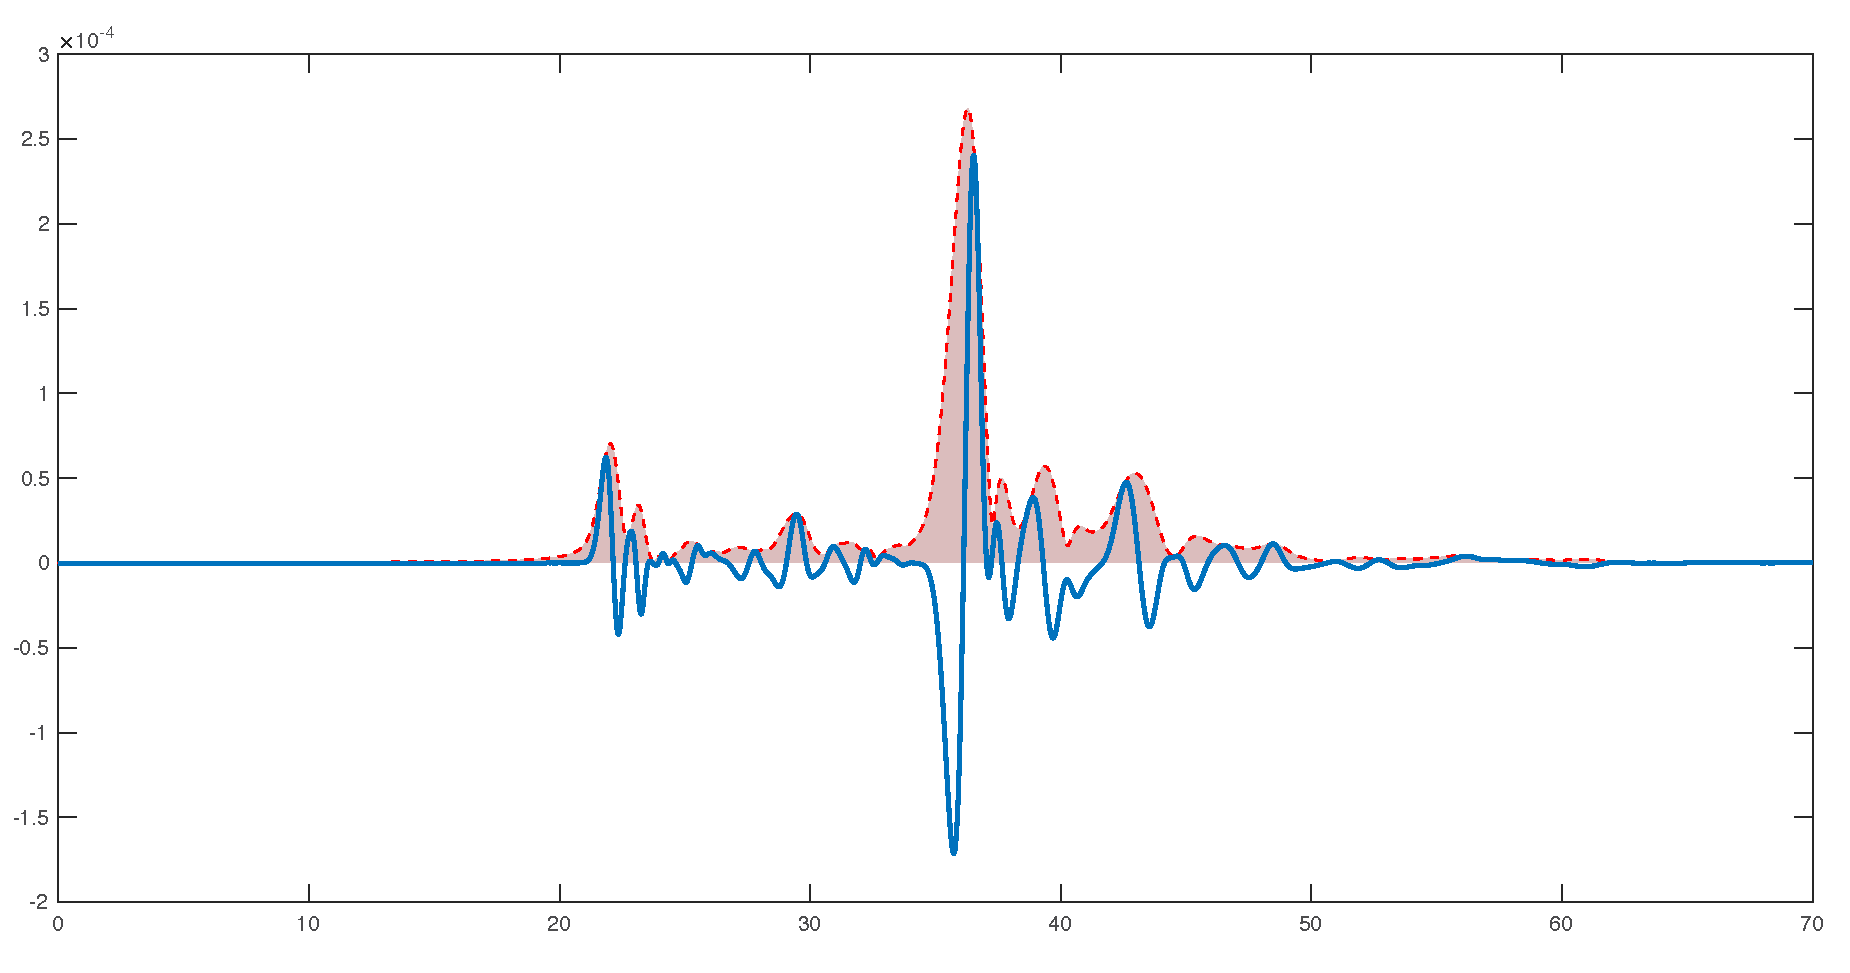
\includegraphics[width=\textwidth]{figures/pdf/signal_envelop.pdf}
    \caption{Example of signal envelop}
    \label{fig:signal_envelop}
\end{figure}


